\section{Déroulement du projet}
\label{sec:deroulement}

\paragraph{Chapeau} Dans cette section, nous décrivons comment le projet a été réalisé en équipe : la répartition des tâches, la synchronisation du travail entre membres de l'équipe, etc.

\subsection{Répartition des tâches}

\begin{center}
\begin{tikzpicture}[
  level 1/.style={sibling distance=50mm},
  edge from parent/.style={->,draw},
  >=latex]

% root of the the initial tree, level 1
\node[root] {Répartition des tâches}
% The first level, as children of the initial tree
  child {node[level 2] (c1) {AYAD Ishak}}
  child {node[level 2] (c2) {Hachoud Rassem}}
  child {node[level 2] (c3) {YAHIAOUI Anis}};

% The second level, relatively positioned nodes
\begin{scope}[every node/.style={level 3}]
\node [below of = c1, xshift=15pt] (c11) {Modélisation UML};
\node [below of = c11] (c12) {Génération};
\node [below of = c12] (c13) {IHM Graphique};
\node [below of = c13] (c14) {Statistiques};
\node [below of = c14] (c15) {Communication};
\node [below of = c15] (c16) {Log4J};
\node [below of = c16] (c17) {Tests Unitaires};

\node [below of = c2, xshift=15pt] (c21) {Modélisation UML};
\node [below of = c21] (c22) {IHM Graphique};
\node [below of = c22] (c23) {Système de Journal};
\node [below of = c23] (c24) {Statistiques};

\node [below of = c3, xshift=15pt] (c31) {Modélisation UML};
\node [below of = c31] (c32) {Génération};
\node [below of = c32] (c33) {IHM Graphique};
\node [below of = c33] (c34) {Mémoire};
\node [below of = c34] (c35) {Chemin des souris};
\end{scope}

% lines from each level 1 node to every one of its "children"
\foreach \value in {1,...,7}
  \draw[->] (c1.195) |- (c1\value.west);

\foreach \value in {1,...,4}
  \draw[->] (c2.195) |- (c2\value.west);

\foreach \value in {1,...,5}
  \draw[->] (c3.195) |- (c3\value.west);
\end{tikzpicture}
\end{center}

\begin{center}
\def\angle{0}
\def\radius{3}
\def\cyclelist{{"orange","blue","red","green"}}
\newcount\cyclecount \cyclecount=-1
\newcount\ind \ind=-1
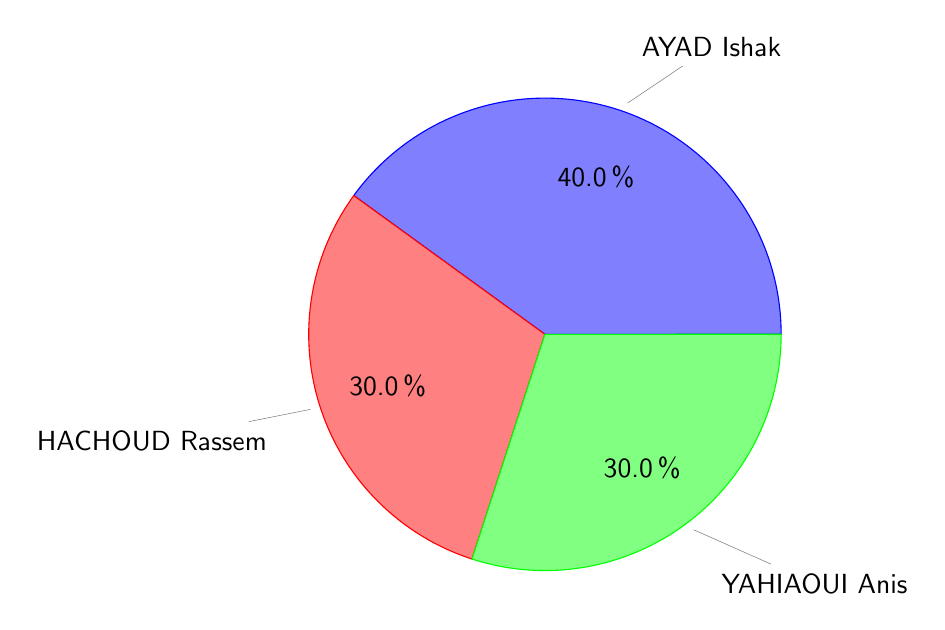
\begin{tikzpicture}[nodes = {font=\sffamily}]
  \foreach \percent/\name in {
      40.0/AYAD Ishak,
      30.0/HACHOUD Rassem,
      30.0/YAHIAOUI Anis,
    } {
      \ifx\percent\empty\else
        \global\advance\cyclecount by 1
        \global\advance\ind by 1
        \ifnum3<\cyclecount
          \global\cyclecount=0
          \global\ind=0
        \fi
        \pgfmathparse{\cyclelist[\the\ind]}
        \edef\color{\pgfmathresult}    
        \draw[fill={\color!50},draw={\color}] (0,0) -- (\angle:\radius)
          arc (\angle:\angle+\percent*3.6:\radius) -- cycle;
        \node at (\angle+0.5*\percent*3.6:0.7*\radius) {\percent\,\%};
        \node[pin=\angle+0.5*\percent*3.6:\name]
          at (\angle+0.5*\percent*3.6:\radius) {};
        \pgfmathparse{\angle+\percent*3.6} 
        \xdef\angle{\pgfmathresult}
        \angle
      \fi
    };
\end{tikzpicture}
\end{center}

\subsection{Synchronisation du travail}
\begin{itemize}
\item Pour la réalisation du projet nous avons utilisé le service web d'hébergement et de gestion de développement de logiciels GitHub pour synchroniser nos travaux.Ce dernier nous a permis d’effectuer des commites à un rythme élevé au commencement du projet pour que tous les membre de l'équipe aient accès aux classes de donnée ,puis après la répartition des tâches le rythme a diminué.
\item Pour la rédaction de ce document nous avons utilisé la plateforme web Overleaf pour répartir les taches, le rythme de rédaction a été très élevé à la fin du projet. 
\end{itemize}

\clearpage
\subsection{Calendrier}
\fig{images/calendar.PNG}{15cm}{10cm}{Calendrier}{cal}
